\documentclass[12pt]{article}
\usepackage{graphicx}

\title{Extracting Data from Shape Files}
\author{Kazi Hasan Zubaer \\ 1105024}
\date{April 12, 2016}

\begin{document}
\maketitle
\section*{Installing QGIS}
QGIS is a software to handle geographic information. The \textit{.shp} file format is a popular file format to represent geographic information and we got road data from Dhaka City Corporation in shape format. To handle the files I used QGIS. It is available on all platforms but works well on Ubuntu. This documentation uses Ubuntu platform. We can install the software directly from the software center for Ubuntu.

\section*{Configuring QGIS}
We will need \textit{MMQGIS} plugin which doesn't come by default with QGIS. To add \textit{MMQGIS} plugin, simply go to plugins $ \rightarrow $ Manage and Install Plugins $ \rightarrow $ Get More. Then search and install \textit{MMQGIS}. To make it work you will need python \textit{xlw} and \textit{xlrd} support. To install these, the easiest way is to install \textit{pip} on your Ubuntu system and then by using \textit{pip} you will be able to install \textit{xlw} and \textit{xlrd}. \\
\begin{figure}
\centering
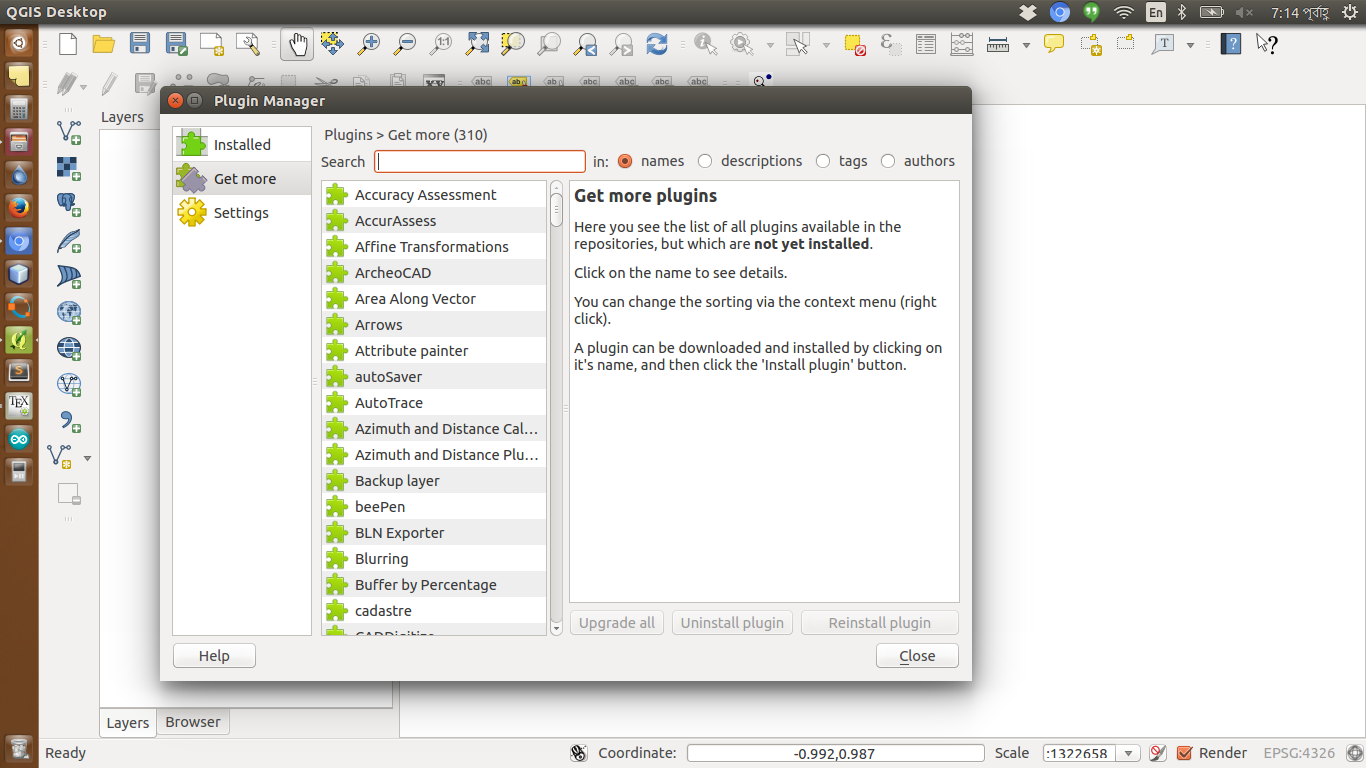
\includegraphics[scale=.25]{qgis01.png}
\caption{Installing new plugins}
\end{figure}

\section*{Loading and Extracting Node from Shape File}
\begin{itemize}
\item Open QGIS and click on \textit{Add Vector} button on the upper left corner. Browse to the shape file.
\item After loading the shape file, choose Vector $ \rightarrow $ Geometry Tools $ \rightarrow $ Extract Nodes. Save the new information in a new shape file (that will be the default option when you will try to extract nodes).
\item  Close the old shape file.
\item Right click on the newly created shape present on the left side of QGIS interface and choose \textit{Open Attribute Table}. You will be able to see some information about the nodes.
\item Choose Vector $ \rightarrow $ Geometry Tools $ \rightarrow $ Export/Add geometry columns. Open the attributes table again. You will be able to see new columns with coordinates of the nodes.
\item Choose MMQGIS $ \rightarrow $ Import/Export $ \rightarrow $ Attributes Export to CSV File. Select ID, ROAD\_TYPE, LENGTH, XCOORD, YCOORD and save the CSV file.
\end{itemize}

\begin{figure}
\centering
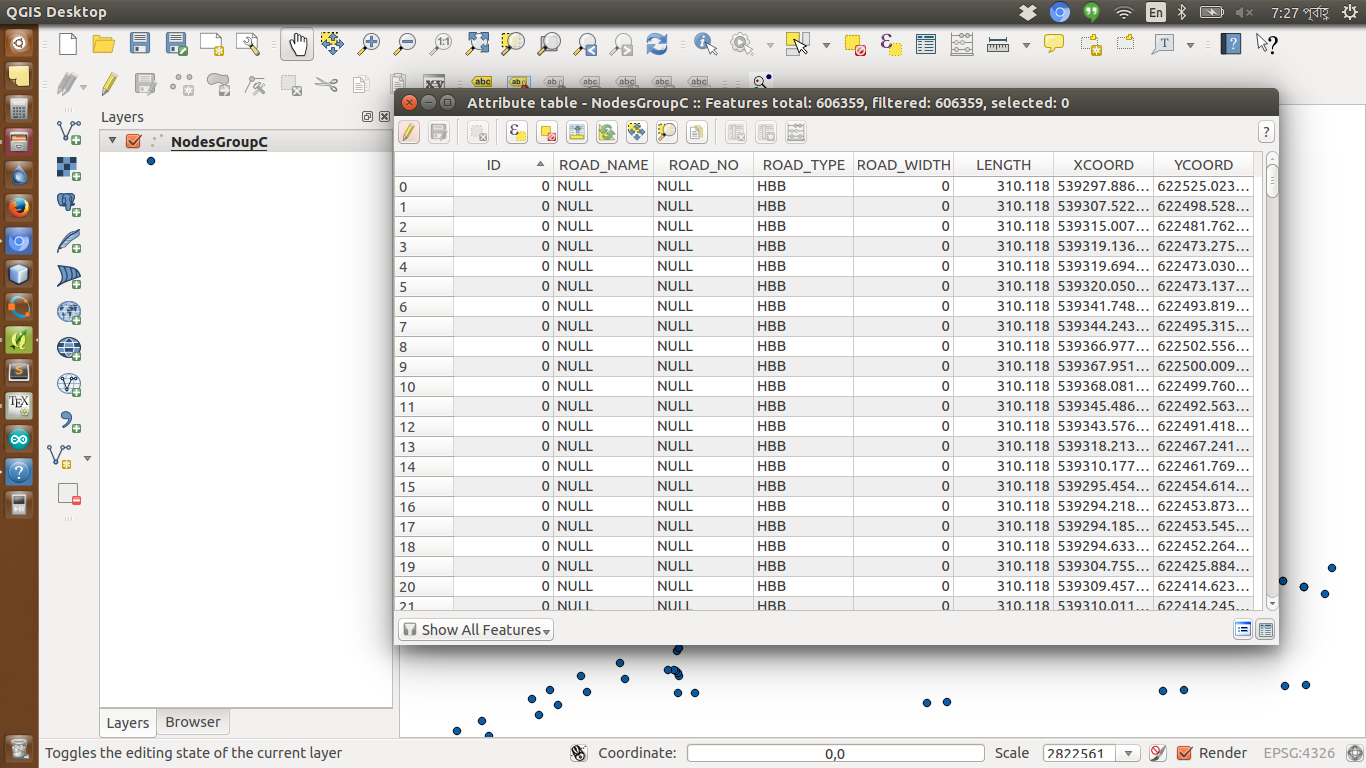
\includegraphics[scale=.25]{qgis02.png}
\caption{Attributes table}
\end{figure}

\begin{figure}
\centering
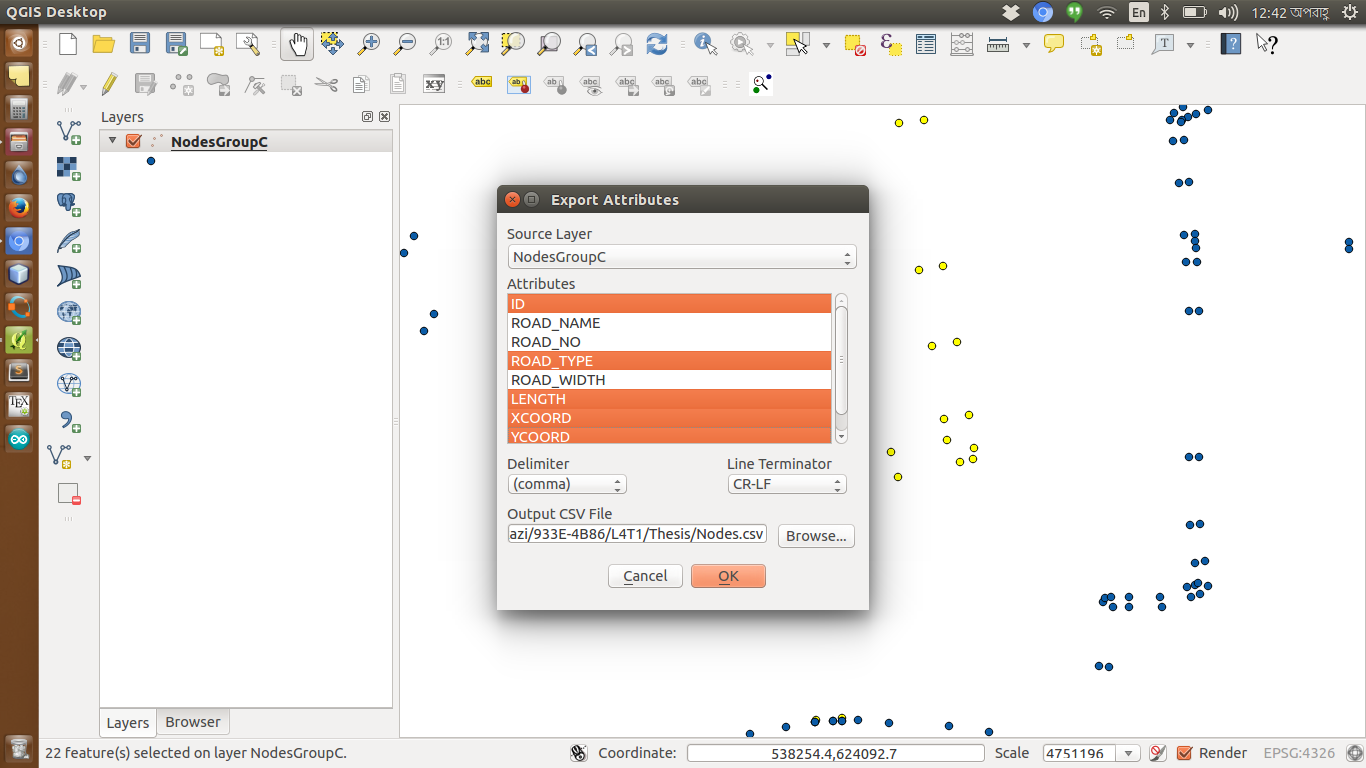
\includegraphics[scale=.25]{qgis03.png}
\caption{Exporting to CSV}
\end{figure}


\section*{Using ShapeParser}
Now we have got a CSV file. The CSV file contains the description of each node. A row represents a node. The row contains the road id the node belongs to, the length of that road, type of the road and coordinates of the node. It has nodes on a road on both sides in a cyclic order. In our simulator, we need nodes on one side of the road in order and the width of the road. Here I have followed the following algorithms to cenvert the information:
\begin{itemize}
\item To find the width, I have calculated the area of a node using \textit{Shoelace theorem}. Then I have divided the area with length.
\item To find points on one side, I have added points one by one. When the length consisted by the added points becomes close to the given length, I have stopped.
\end{itemize}

If we keep the CSV file in the project folder of \textit{ShapeParser} and run the program, it will generate a text file with columns ROAD\_ID,WIDTH,XCOORD,YCOORD.\\

The description of defferent classes of \textit{ShapeParser} is given below:
\subsection*{Point Class}
This class mainly represents a geometric point. We have member methods to find its magnitude and distance from another point.

\subsection*{Road Class}
The road class has following member variables:
\begin{itemize}
\item \textit{id}, the id of the road.
\item \textit{n}, number of points on original description (Points on both side of the road).
\item \textit{width} and \textit{length}, width and length of the raod.
\item \textit{ptsRaw}, point array to hold points on both sides of the road.
\item \textit{ptsFinal}, points on one side of the road.\\
\end{itemize}

The road class has the followint member methods:
\begin{itemize}
\item \textit{Road}, the constructor.
\item \textit{Calculate}, to calculate the width and ptsFinal.
\item \textit{getID, getWidth, getpoints - }, getter methods.
\end{itemize}

\subsection*{ShapeParser Class}
The driver class which handles the input and output. Modify the name of the input and output files here according to your input and output file name. I have ignored roads with ROAD\_TYPE \textit{Katcha}. Include the roads if necessary by changing the corresponding part of this class. 
\end{document}
